\documentclass{article}
\usepackage{amsmath,amsthm,amssymb,amsfonts}
\usepackage{setspace,enumitem}
\usepackage{graphicx}
\usepackage{hyperref}
\usepackage{natbib}
\usepackage{lscape}
\usepackage{afterpage}
\usepackage{xcolor}
\usepackage{etoolbox}
\usepackage{booktabs}
\usepackage{pdfpages}
\usepackage{multicol}
\usepackage{geometry}
\usepackage{accents}
\usepackage{bbm}
\usepackage{verbatim}
\usepackage{lscape}

\setlength{\parindent}{0cm}
\geometry{margin = 1in}

\newcommand{\R}{\mathbb{R}}
\newcommand{\ubar}[1]{\underaccent{\bar}{#1}}
\newcommand{\Int}{\text{Int}}
\newcommand{\xbf}{\mathbf{x}}
\newcommand{\Abf}{\mathbf{A}}
\newcommand{\Bbf}{\mathbf{B}}
\newcommand{\Gbf}{\mathbf{G}}
\newcommand{\bbf}{\mathbf{b}}
\newcommand{\one}{\mathbbm{1}}

\newtoggle{extended}
\settoggle{extended}{false}

\title{ECON 717A: Problem Set 2}
\author{Alex von Hafften }

\begin{document}

\maketitle

\section{Write-Up}

\subsection*{Problem 0}

I drop observations with \texttt{sample} equal to 3.  This step dropped 2,490 observations.

\subsection*{Problem 1}

I regressed earnings in 1978 on treatment with and without the covariate of age, age squared, education, indicators for black, Hispanic, married, and no degree, and earnings in 1974 and 1975.  The treatment effect is \$886.30 without covariates and \$818.70 with covariates with both statistically significant at the 10 percent level.  It is important to include covariate even in experimental data because we get a more precise estimate for the treatment effect.

\begin{center}
\documentclass[]{article}
\setlength{\pdfpagewidth}{8.5in} \setlength{\pdfpageheight}{11in}
\begin{document}
\begin{tabular}{lcc} \hline
 & (1) & (2) \\
VARIABLES & m\_equity\_compustat & m\_equity\_compustat \\ \hline
 &  &  \\
m\_equity\_crsp & 1.050*** & 1.050*** \\
 & (0.00701) & (0.00701) \\
Constant & 108.4*** & 108.4*** \\
 & (19.05) & (19.05) \\
 &  &  \\
Observations & 16,263 & 16,263 \\
 R-squared & 0.580 & 0.580 \\ \hline
\multicolumn{3}{c}{ Standard errors in parentheses} \\
\multicolumn{3}{c}{ *** p$<$0.01, ** p$<$0.05, * p$<$0.1} \\
\end{tabular}
\end{document}

\end{center}

\pagebreak

\subsection*{Problem 2}

I drop observations with \texttt{sample} equal to 1 and \texttt{treated} equal to 1.  This step dropped 297 observations.

\subsection*{Problem 3}

I define \texttt{in\_control} equal to one if \texttt{sample} equals one and zero otherwise.  The probit estimation for the propensity scores are the coarse scores and the rich scores are below.

\begin{center}
\begin{tabular}{lcc} \hline
 & (1) & (2) \\
VARIABLES & in\_control & in\_control \\ \hline
 &  &  \\
age & 0.253*** & 0.322*** \\
 & (0.0293) & (0.0316) \\
age\_2 & -0.00453*** & -0.00548*** \\
 & (0.000493) & (0.000530) \\
educ & 0.0169 & 0.0178 \\
 & (0.0181) & (0.0183) \\
black & 1.990*** & 1.950*** \\
 & (0.0778) & (0.0796) \\
hisp & 0.973*** & 0.978*** \\
 & (0.103) & (0.106) \\
married & -1.101*** & -0.909*** \\
 & (0.0826) & (0.0869) \\
nodegree & 1.133*** & 1.071*** \\
 & (0.100) & (0.104) \\
re74 &  & -1.07e-06 \\
 &  & (8.60e-06) \\
re75 &  & -5.76e-05*** \\
 &  & (9.56e-06) \\
Constant & -6.358*** & -7.108*** \\
 & (0.483) & (0.509) \\
 &  &  \\
Observations & 16,417 & 16,417 \\
Failures completely determined & 727 & 1359 \\
 Successes completely determined & 0 & 0 \\ \hline
\multicolumn{3}{c}{ Standard errors in parentheses} \\
\multicolumn{3}{c}{ *** p$<$0.01, ** p$<$0.05, * p$<$0.1} \\
\end{tabular}

\end{center}

The completely determined observations are 727 and 1359 comparison group observations that have propensity scores with almost zero.

\pagebreak

\subsection*{Problem 4}

The table below shows descriptive statistics of \texttt{pscorea} and \texttt{pscoreb}.

\begin{center}
{
\def\sym#1{\ifmmode^{#1}\else\(^{#1}\)\fi}
\begin{tabular}{l*{1}{cccccc}}
\hline\hline
                    &        Mean&          SD&         Min&      Median&         Max&           N\\
\hline
0                   &        0.02&        0.07&        0.00&        0.00&        0.69&      15,992\\
1                   &        0.39&        0.23&        0.00&        0.47&        0.69&         425\\
Total               &        0.03&        0.09&        0.00&        0.00&        0.69&      16,417\\
\hline\hline
\end{tabular}
}

\end{center}

\begin{center}
{
\def\sym#1{\ifmmode^{#1}\else\(^{#1}\)\fi}
\begin{tabular}{l*{1}{cccccc}}
\hline\hline
                    &        Mean&          SD&         Min&      Median&         Max&           N\\
\hline
0                   &        0.02&        0.06&        0.00&        0.00&        0.79&      15,992\\
1                   &        0.42&        0.25&        0.00&        0.46&        0.80&         425\\
Total               &        0.03&        0.10&        0.00&        0.00&        0.80&      16,417\\
\hline\hline
\end{tabular}
}

\end{center}

These descriptive statistics suggest that imposing the common support condition will not drop many observations.  For \texttt{pscorea}, the minimum is zero for both groups and the maximum is 0.69 for both groups.  This suggests that there are compared observations within the comparison group to the control group.  Similarly for \texttt{pscoreb}, the minimum is zero for both groups and the maximum is around 0.8 for both groups. These descriptive statistics suggest that the CPS group is not very comparable to the experimental control group.  That is, these descriptive statistics highlight the importance of matching because the control group has a much higher mean propensity score than the comparison group (i.e., 0.39 vs. 0.02 for \texttt{pscorea} and 0.42 vs. 0.02 for \texttt{proscoreb}).

\subsection*{Problem 5}

Below are histograms (based on the provided code) for \texttt{pscorea} and \texttt{pscoreb} across the CPS comparison group (i.e., 0) and the experimental control group (i.e., 1) with and without the lowest bin (i.e., \texttt{pscorex} $\in (0.0, 0.05)$). Looking at the first two histograms, most of the comparison group observations have a very low estimated propensity score (confirming the descriptive statistics), so the comparison group is not very comparable to the control group. I added histograms without the lowest bin because many observations in the comparison group have estimated propensity scores of basically zero impairing our ability to evaluate the common support condition.  Looking at the second two histograms, the common support condition seems to be well satisfied with comparison group observations at all propensity levels of the control group. These histograms highlight concerns about matching without replacement because the number of observations in the control group with high propensity scores is larger than the number of observations in the comparison group with large propensity scores (i.e. on the right of the graphs the red bars are taller than the blue bars).  Matching without replacement would cause these the control group observations to be matched with comparison group observations with significantly lower propensity scores.

\begin{center}
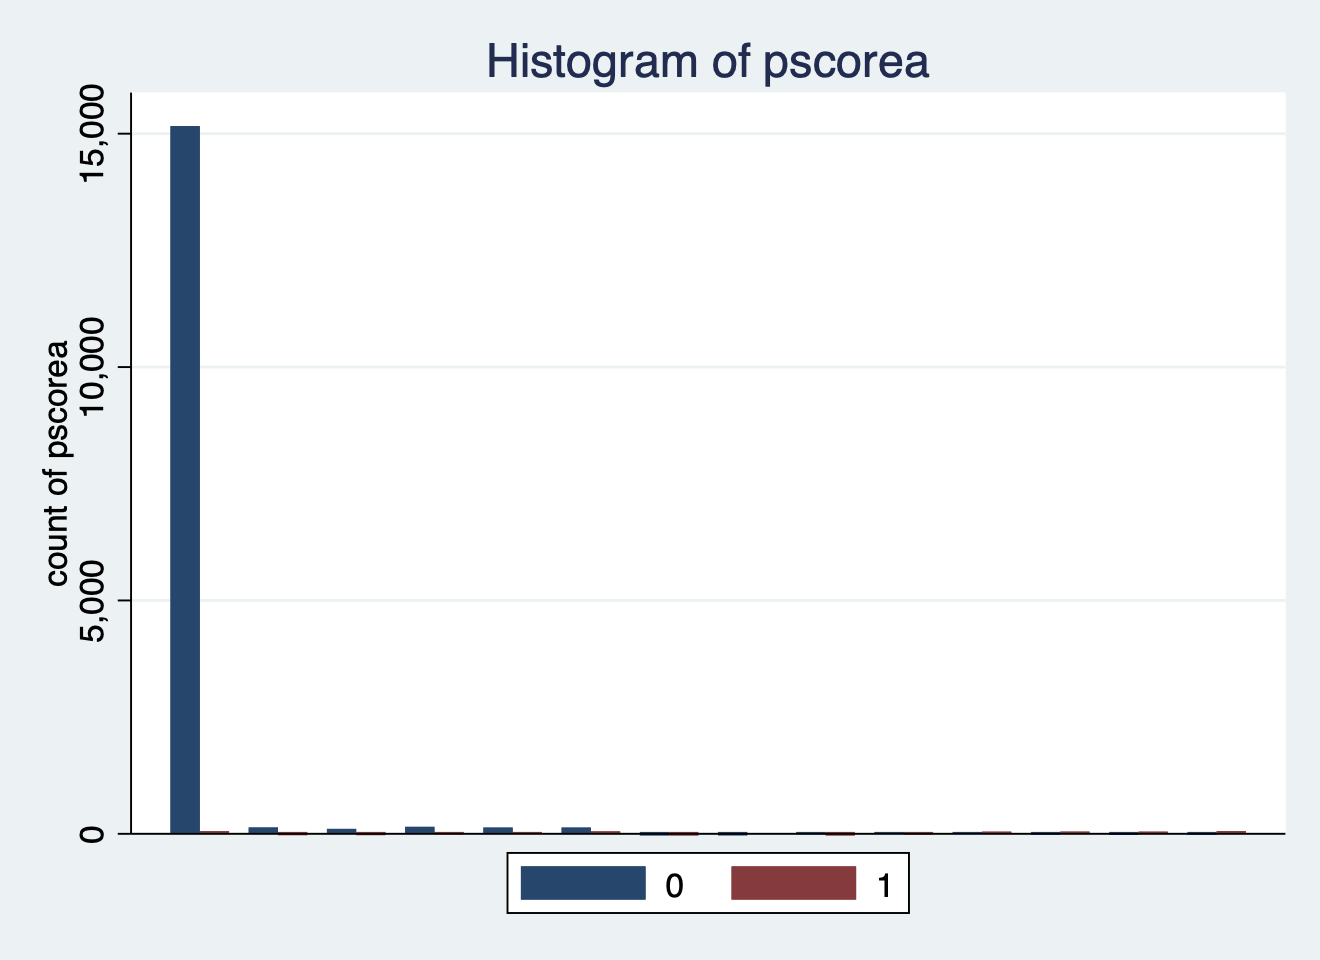
\includegraphics[scale = 0.5]{figure_5a}
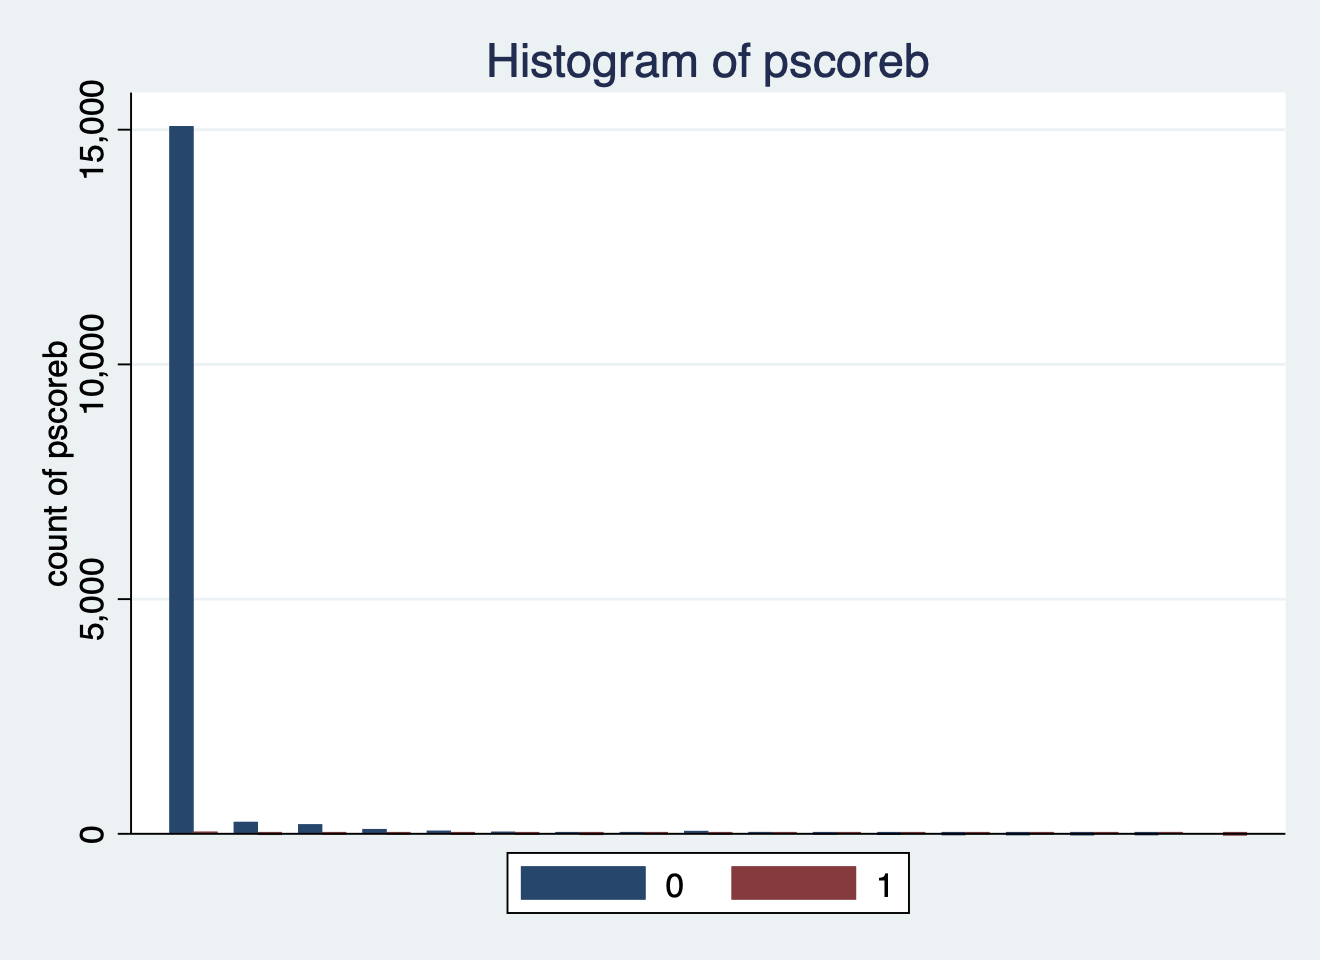
\includegraphics[scale = 0.5]{figure_5b}
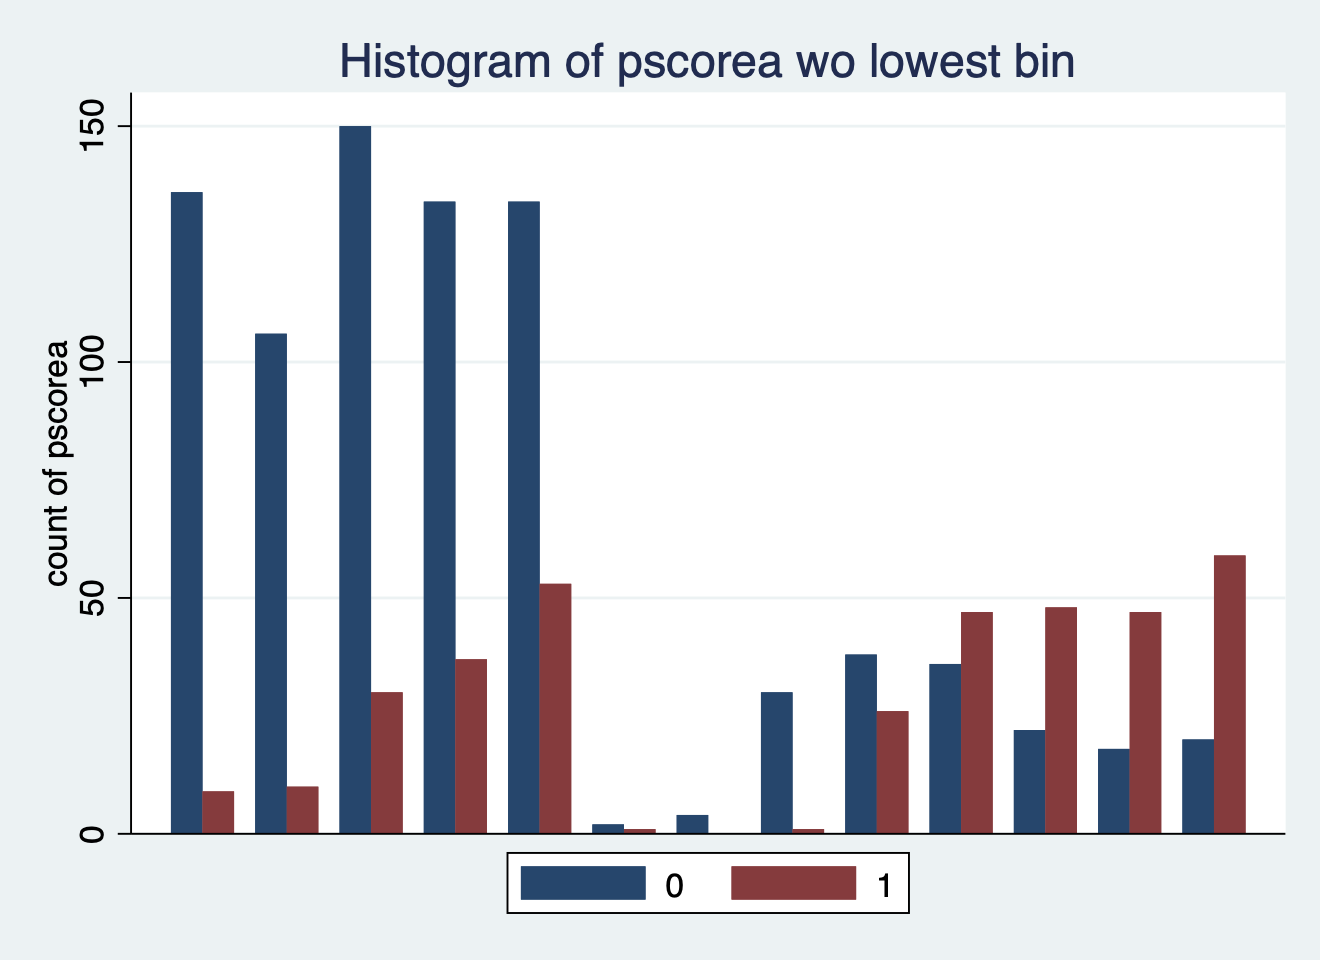
\includegraphics[scale = 0.5]{figure_5a_2}
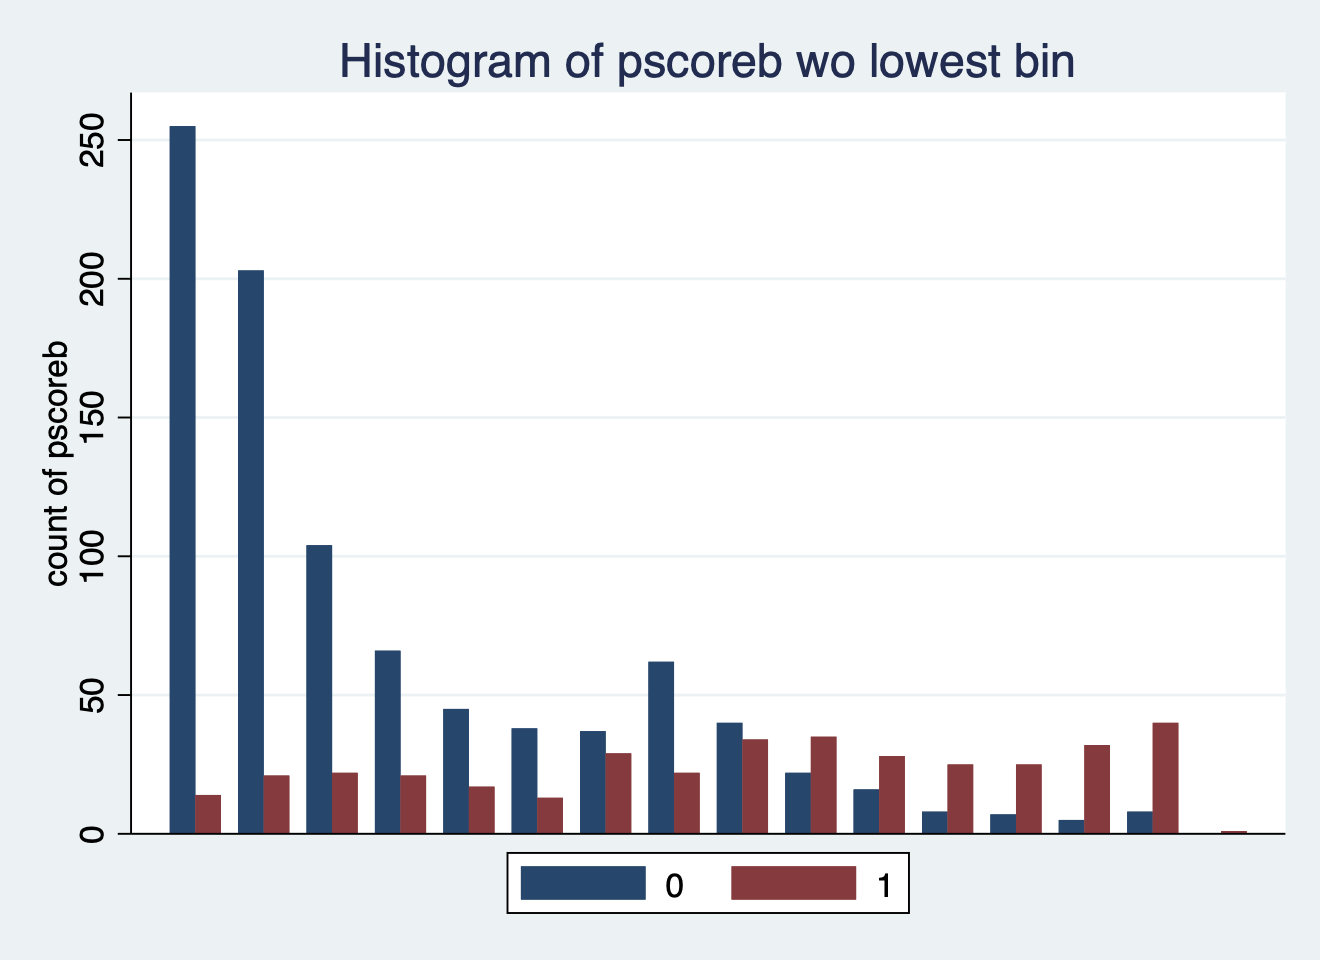
\includegraphics[scale = 0.5]{figure_5b_2}
\end{center}

\pagebreak

\subsection*{Problem 6}

Using single nearest neighbor matching without replacement and common support condition, I estimate the non-experimental bias reported in the table below.  The non-experimental bias is significant and negative indicating that even after matching observations in the control group that significantly lower earnings in 1978.  The non-experimental bias is lower when matching based on the rich propensity scores.  No observations are dropped when matching with coarse propensity scores.  Seven observations are dropped when matching with fine propensity scores.

\begin{center}
\begin{tabular}{lc} \hline
 & (1) \\
VARIABLES & rate18\_20ht \\ \hline
 &  \\
mlda21 & 5.755*** \\
 & (1.669) \\
 &  \\
Observations & 651 \\
R-squared & 0.691 \\
Fixed Effects & State and Year \\
 Clusters & None \\ \hline
\multicolumn{2}{c}{ Robust standard errors in parentheses} \\
\multicolumn{2}{c}{ *** p$<$0.01, ** p$<$0.05, * p$<$0.1} \\
\end{tabular}

\end{center}

\subsection*{Problem 7}

Using single nearest neighbor matching with replacement and common support condition, I estimate the non-experimental bias reported in the table below.  The non-experimental bias is still significant and negative but it is lower than without replacement.  As mentioned in problem 5, this reduction in the non-experimental bias is due the relatively fewer comparison group observations with high propensity scores, so that there's more non-experimental bias when matching without replacement.

\begin{center}
\begin{table}[h!]
\begin{center}
\begin{tabular}{lrrr}
\toprule
& Unmatched & ATT for \texttt{pscorea} & ATT for \texttt{pscoreb}  \\
\hline
Difference & -9756.610000000001 & -3677.03 & -1515.99 \\
SE & 470.16 & 934.5 & 707.62 \\
\bottomrule
\end{tabular}
\end{center}
\end{table}

\end{center}

\subsection*{Problem 8}
\subsection*{Problem 9}

\begin{center}
\begin{tabular}{lccc} \hline
 & (1) & (2) & (3) \\
VARIABLES & Michigan & Maryland & Maryland \\ \hline
 &  &  &  \\
mlda21\_mi & -1.006 &  &  \\
 & (3.746) &  &  \\
mlda21\_md &  & 7.652* & 7.652* \\
 &  & (3.915) & (3.915) \\
 &  &  &  \\
Observations & 403 & 403 & 403 \\
R-squared & 0.716 & 0.719 & 0.719 \\
 Fixed Effects & State and Year & State and Year & State and Year \\ \hline
\multicolumn{4}{c}{ Robust standard errors in parentheses} \\
\multicolumn{4}{c}{ *** p$<$0.01, ** p$<$0.05, * p$<$0.1} \\
\end{tabular}

\end{center}

\subsection*{Problem 10}


\begin{center}
\begin{tabular}{lc} \hline
 & (1) \\
VARIABLES & rate18\_20ht \\ \hline
 &  \\
mlda21\_14 & 1.705 \\
 & (3.252) \\
mlda\_later & 7.260 \\
 & (5.415) \\
 &  \\
Observations & 651 \\
R-squared & 0.695 \\
 Fixed Effects & State and Year \\ \hline
\multicolumn{2}{c}{ Robust standard errors in parentheses} \\
\multicolumn{2}{c}{ *** p$<$0.01, ** p$<$0.05, * p$<$0.1} \\
\end{tabular}

\end{center}

\subsection*{Problem 11}

\begin{center}
\begin{tabular}{lc} \hline
 & (1) \\
VARIABLES & re78 \\ \hline
 &  \\
in\_control & -1,853*** \\
 & (343.2) \\
age & -235.5*** \\
 & (40.08) \\
age\_2 & 1.858*** \\
 & (0.550) \\
educ & 163.3*** \\
 & (28.53) \\
black & -832.4*** \\
 & (193.9) \\
hisp & -114.2 \\
 & (213.9) \\
married & 199.4 \\
 & (150.8) \\
nodegree & 296.6* \\
 & (174.3) \\
re74 & 0.291*** \\
 & (0.0152) \\
re75 & 0.471*** \\
 & (0.0153) \\
Constant & 7,757*** \\
 & (726.7) \\
 &  \\
Observations & 16,417 \\
 R-squared & 0.483 \\ \hline
\multicolumn{2}{c}{ Robust standard errors in parentheses} \\
\multicolumn{2}{c}{ *** p$<$0.01, ** p$<$0.05, * p$<$0.1} \\
\end{tabular}

\end{center}


\subsection*{Problem 12}

\begin{center}
\begin{tabular}{lc} \hline
 & (1) \\
VARIABLES & re78 \\ \hline
 &  \\
age & -252.0*** \\
 & (40.92) \\
age\_2 & 2.041*** \\
 & (0.561) \\
educ & 166.6*** \\
 & (28.79) \\
black & -773.9*** \\
 & (199.6) \\
hisp & -168.2 \\
 & (218.9) \\
married & 244.1 \\
 & (153.1) \\
nodegree & 330.7* \\
 & (176.9) \\
re74 & 0.299*** \\
 & (0.0152) \\
re75 & 0.470*** \\
 & (0.0153) \\
Constant & 7,908*** \\
 & (739.7) \\
 &  \\
Observations & 15,992 \\
 R-squared & 0.476 \\ \hline
\multicolumn{2}{c}{ Robust standard errors in parentheses} \\
\multicolumn{2}{c}{ *** p$<$0.01, ** p$<$0.05, * p$<$0.1} \\
\end{tabular}

\end{center}

\begin{center}
{
\def\sym#1{\ifmmode^{#1}\else\(^{#1}\)\fi}
\begin{tabular}{l*{1}{cccccc}}
\hline\hline
                    &        Mean&          SD&         Min&      Median&         Max&           N\\
\hline
0                   &   14,846.66&    6,654.46&      162.96&   15,370.95&   25,693.43&      15,992\\
1                   &    6,941.60&    4,269.45&      275.72&    5,770.59&   33,124.62&         425\\
Total               &   14,642.01&    6,721.77&      162.96&   15,110.59&   33,124.62&      16,417\\
\hline\hline
\end{tabular}
}

\end{center}

\subsection*{Problem 13}

%\pagebreak
%\begin{landscape}
%\section{Stata Log File}
%\verbatiminput{analysis.log}
%\end{landscape}

\end{document}

